\documentclass[inverse]{../slidedeck}
\newcommand*\thetitle{README}
\newcommand*\thesubtitle{vs. IEEE, RUP, SWEBOK, CMMI}
\sdTopLeft{@yegor256}
\sdBottomLeft{Lecture \#1: \thetitle{} \thesubtitle{}}
\begin{document}

\sdTitle{\thetitle}{\thesubtitle}

\sdClear

\sdToc{Software vs. Interiors}\sdClick
\sdToc{IEEE 1016}\sdClick
\sdToc{SAD \@ RUP}\sdClick
\sdToc{TS \@ CMMI}\sdClick
\sdToc{SWEBOK}\sdClick
\sdToc{README}\sdClick
\sdToc{Books, Venues, C2A}

\sdClear

\sdTocNext
\sdQuote{freeman}{Design encompasses all the activities involved in conceptualizing, framing, implementing, commissioning, and ultimately modifying complex systems—not just the activity following requirements specification and before programming, as it might be translated from a stylized software engineering process.}{Peter Freeman and David Hart\newline CACM vol. 47, no. 8, 2004}

\sdClear

\sdBanner{Software Design \newline Description (SDD)}
\sdClear

\sdMenu{Glossary}
\sdMenu{Languages}
\sdMenu{Stakeholders}
\sdMenu{Concerns}
\sdMenu{Viewpoints}
\sdMenu{Elements}
\sdMenu{Rationale}

% Glossary
\sdPrint{
  A request is data package sent from a client to a server.
  A client is a computer with a web browser.
  A server is a computer with a software installed.
}
\sdBanner[green,M]{If I don't understand you, it's your fault!}
\sdQR{https://www.yegor256.com/2015/03/16/technical-glossaries.html}

% Languages
\sdClear
\sdMenuNext
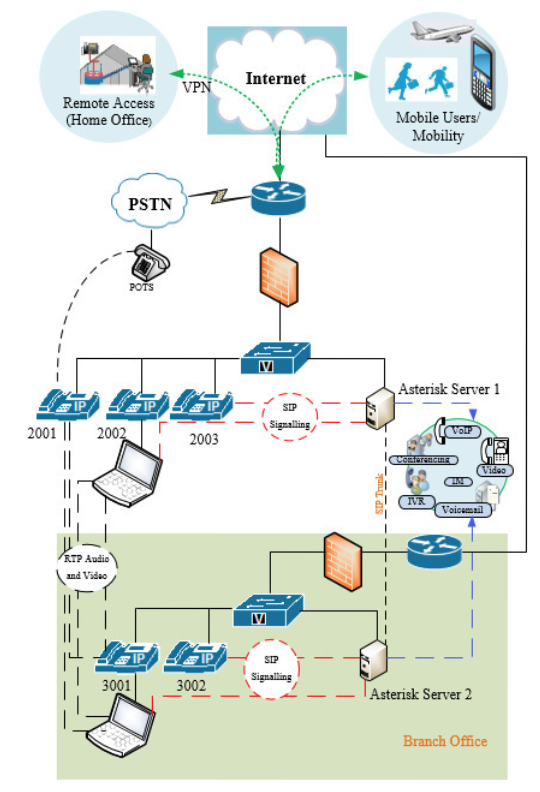
\includegraphics[width=0.75\textwidth]{bad-diagram}\par
UML + visual-paradigm.com

% Stakeholders
\sdClear
\sdMenuNext
\sdQuote{pmbok}{Identify Stakeholders is the process of identifying the people, groups, or organizations that could impact or be impacted by a decision, activity, or outcome of the project.}{A Guide to the Project Management Body of Knowledge (PMBOK Guide), Project Stakeholder Management Knowledge Area}

% Concerns
\sdClear
\sdMenuNext
Functional and Non-Functional Requirements

% Viewpoints
\sdClear
\sdMenuNext
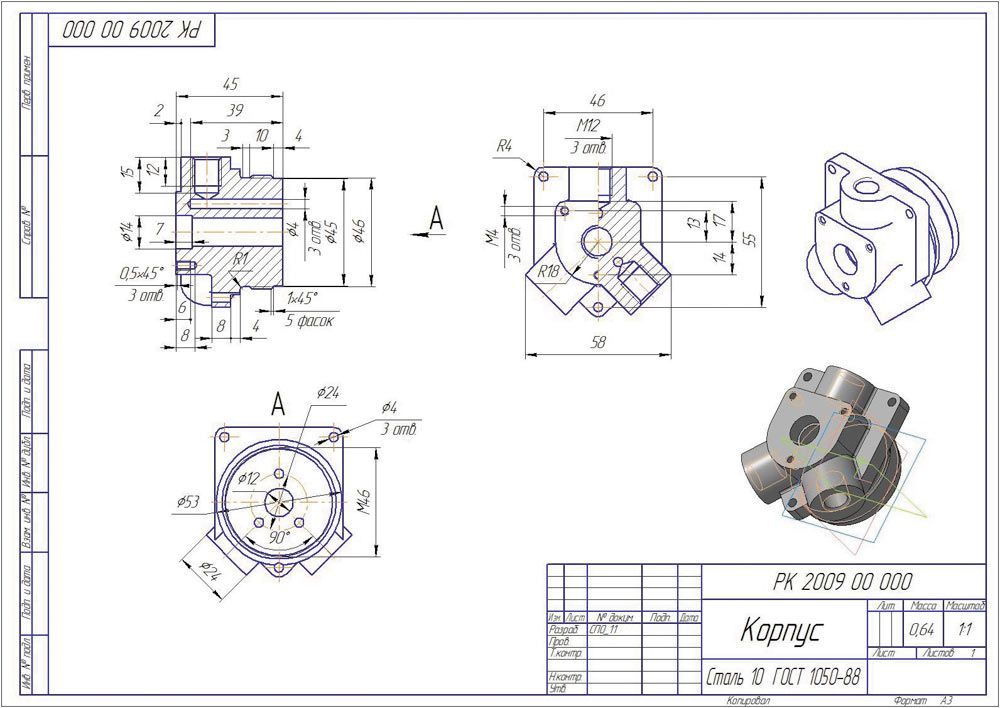
\includegraphics[width=0.7\textwidth]{viewpoint}

% Elements
\sdClear
\sdMenuNext
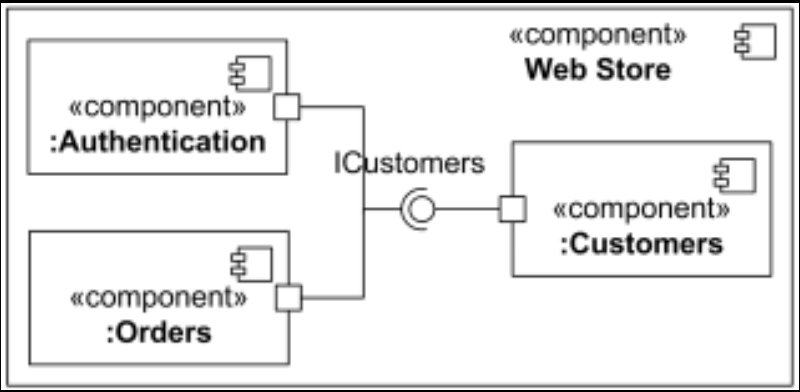
\includegraphics[width=0.7\textwidth]{element}

% Rationale
\sdClear
\sdMenuNext
\sdBanner[green,M]{Why MongoDB, why not MySQL?}
Multi-Criteria Decision Making (MCDM)\par
Architecture Tradeoff Analysis Method (ATAM)\par
Decision Table\par
Multi Factor Analysis\par
Decision Matrix

\sdClear
\sdMenuDelete

\sdQuote{cmmi}{Detailed design is focused on software product component development. The internal structure of product components is defined, data schemas are generated, algorithms are developed, and heuristics are established to provide product component capabilities that satisfy allocated requirements.}{CMMI for Development \par Capability Maturity Model Integration (CMMI) \par Technical Solution (TS) Process Area}

\end{document}
